\documentclass[11pt]{beamer}
\usetheme{Rochester}
\usepackage[utf8]{inputenc}
\usepackage{amsmath}
\usepackage{amsfonts}
\usepackage{amssymb}
\usepackage{graphicx}
%\author{}
%\title{}
%\setbeamercovered{transparent} 
%\setbeamertemplate{navigation symbols}{} 
%\logo{} 
%\institute{} 
%\date{} 
%\subject{} 
\begin{document}

\begin{frame}
\title{Computational Astrophysics}
\author{E. Larrañaga}
\institute{Observatorio Astronómico Nacional\\
Universidad Nacional de Colombia}
\titlepage
\end{frame}

\begin{frame}{Outline}
\tableofcontents
\end{frame}

\section{Interpolation}

\begin{frame}[fragile]{Interpolation}
We know the values of a function $f$ only at discrete locations $x_i$, but want to
know its values at general points $x$.
\begin{figure}
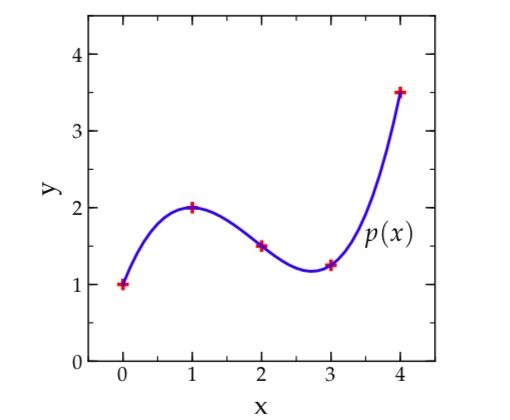
\includegraphics[scale=0.3]{interpolation.jpeg}
\end{figure}
\end{frame}

\begin{frame}[fragile]{Interpolation}
We  look for an approximation
$p(x)$ that uses the discrete information about $f(x)$ at $x_i$ to
interpolate $f(x)$ between the $x_i$ with $p(x_i) = f(x_i)$. \\
\pause
\bigskip 

If $x$ is
outside $[x_\mathrm{min},x_\mathrm{max}]$, where $x_\mathrm{min} =
\min \{x_i; \forall i\}$ and $x_\mathrm{max} = \max \{x_i; \forall i\}$,
$p(x)$ extrapolates $f(x)$.
\end{frame}

\subsubsection{Linear Interpolation}
\begin{frame}[fragile]{Linear Interpolation}

We obtain the linear approximation $p(x)$ for $f(x)$ in the interval
$[x_i,x_{i+1}]$ by 
\begin{equation}
\label{eq:linterp}
p(x) = f(x_i) +\!\!\! \underbrace{\frac{f(x_{i+1}) - f(x_i)}{x_{i+1} -
    x_i}}_\text{1st-order forward difference}\!\!\! (x-x_i) +
\mathcal{O}(h^2)\,,
\end{equation}
where $h = x_{i+1} - x_i$. \\
\bigskip
\pause

The interpolated function can be differentiated once, but
the derivative will be discontinuous at $x_{i+1}$ and
$x_i$.
\end{frame}


\subsubsection{Quadratic Interpolation}
\begin{frame}[fragile]{Quadratic Interpolation}

The quadratic approximation $p(x)$ for $f(x)$ in the interval
$[x_{i},x_{i+1}]$ is given by
\begin{equation}
\begin{aligned}
p(x) &= \frac{(x-x_{i+1})(x-x_{i+2})}{(x_i - x_{i+1})(x_i - x_{i+2})} f(x_i)\\
&+ \frac{(x-x_{i})(x-x_{i+2})}{(x_{i+1} - x_{i})(x_{i+1} - x_{i+2})} f(x_{i+1})\\
&+ \frac{(x-x_i)(x-x_{i+1})}{(x_{i+2} - x_i)(x_{i+2} - x_{i+1})} f(x_{i+2})\\
&+ \mathcal{O}(h^3)\,,
\end{aligned}
\end{equation}
where $h = \max\{x_{i+2}-x_{i+1},x_{i+1}-x_i\}$.\\

\pause
\bigskip

$p(x)$ is twice differentiable. Its first derivative will be continuous,
but $p''(x)$ will have finite-size steps.
\end{frame}

\subsubsection{Lagrange Interpolation}
\begin{frame}[fragile]{Lagrange Interpolation}
\emph{Lagrange Interpolation} provides a means of constructing
general interpolating polynomials of degree $n$ using data at $n+1$
points.\\

\pause
Consider linear interpolation rewritten as
\begin{equation}
\begin{aligned}
f(x) \approx p(x) & = \frac{x-x_{i+1}}{x_i - x_{i+1}} f(x_i) +
\frac{x-x_i}{x_{i+1}-x_i} f(x_{i+1}) + \mathcal{O}(h^2)\,,\\
  & = \sum_{j=i}^{i+1} f(x_j) L_{1j}(x) + \mathcal{O}(h^2)\,,\\
& \text{where}\,\, L_{1j}(x) = \frac{x-x_k}{x_j-x_k}\bigg|_{k\ne j}\,.
\end{aligned}
\end{equation}
\end{frame}

\begin{frame}[fragile]{Lagrange Interpolation}
This is generalized this to an $n$-th degree polynomial that
passes through all $n+1$ data points:
\begin{equation}
p(x) = \sum_{j=0}^{n} f(x_j) L_{nj}(x) + \mathcal{O}(h^{n+1})\,,
\end{equation}
with
\begin{equation}
L_{nj}(x) = \prod_{k\ne j}^{n} \frac{x-x_k}{x_j - x_k}\,.
\end{equation}

Note that this clearly satisfies the interpolating condition,
$p(x_i) = f(x_i)$.

\end{frame}

\begin{frame}[fragile]{Lagrange Interpolation}
\begin{figure}
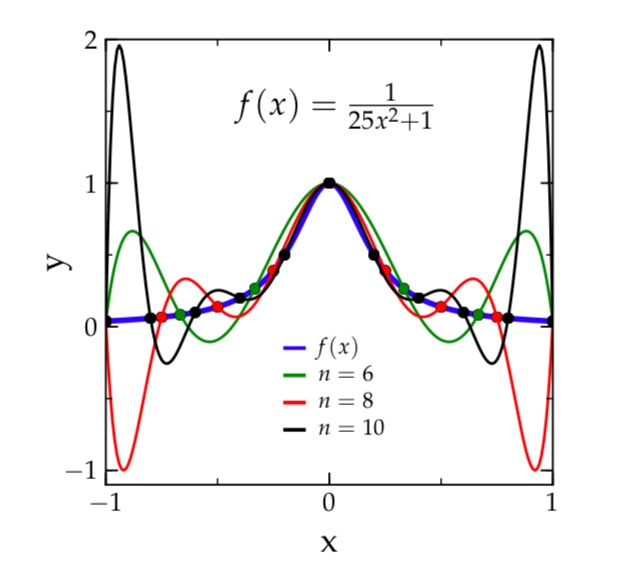
\includegraphics[scale=0.3]{interpolationExample.jpeg}
\end{figure}

\end{frame}



\end{document}